\documentclass[11pt]{article}
% Adapted from an original template by Hlyni Arnórssyni,
% Reykjavik University, Iceland

% ------------------------------ PAGE SETTINGS ------------------------------
\usepackage{geometry}

\geometry{
    paper=a4paper,
    top=2.5cm,
    bottom=2.5cm,
    left=2.5cm,
    right=2.4cm,
    headheight=0.75cm,
    footskip=1.5cm,
    headsep=0.75cm
}

% ------------------------------ BASIC PACKAGES ------------------------------
\usepackage{blindtext}

% Character encoding
\usepackage[T1]{fontenc}
\usepackage[utf8]{inputenc}

% Mathematics
\usepackage{amsmath, amsfonts, amsthm, amssymb}
\usepackage{braket, nicefrac}

% SI units
\usepackage{siunitx}

% Lists / columns
\usepackage{enumitem, multicol}

% ------------------------------ FIGURES ------------------------------
\usepackage{graphicx}
\usepackage{float}
\usepackage{keystroke}
\usepackage{pgfplots}
\usepgfplotslibrary{units}
\pgfplotsset{compat=1.16}

% Search these locations automatically for figures
\graphicspath{{fig/}{graphics/}{Graphics/}{./}}

% ------------------------------ TABLES ------------------------------
\usepackage{tabularx}
\usepackage{array}
\usepackage[table]{xcolor}

% ------------------------------ TYPOGRAPHY ------------------------------
\usepackage{caption}
\usepackage{titlesec}
\usepackage{microtype}
\usepackage{csquotes}

% ------------------------------ COLORS ------------------------------
\definecolor{GWBlue}{HTML}{1E4E79}

% ------------------------------ SECTION STYLING ------------------------------
\titleformat{\section}
  {\Large\bfseries\color{GWBlue}}
  {\thesection.}
  {0.40em}
  {}

\titlespacing*{\section}
  {0pt}
  {0.70em}
  {0.28em}

% ------------------------------ CAPTION STYLING ------------------------------
\captionsetup{
    font=small,
    labelfont=bf,
    textfont=it,
    labelsep=period,
    skip=4pt
}

% ------------------------------ PARAGRAPH SPACING ------------------------------
\setlength{\parindent}{0pt}
\setlength{\parskip}{0.30em}

% ------------------------------ BIBLIOGRAPHY ------------------------------
\usepackage[
    backend=biber,
    style=authoryear,
    sorting=none,
    giveninits=true,
    maxbibnames=99,
    dashed=false
]{biblatex}

\addbibresource{references.bib}

\DeclareNameAlias{sortname}{family-given}
\DeclareNameAlias{default}{family-given}
\DeclareFieldFormat[article]{title}{#1}
\DeclareFieldFormat[misc]{title}{#1}
\renewbibmacro{in:}{}

\AtEveryBibitem{%
    \clearfield{doi}%
    \clearfield{urldate}%
}

\AtBeginBibliography{\small}
\setlength{\bibitemsep}{0.35em}

% ------------------------------ HYPERLINKS ------------------------------
\usepackage{hyperref}

\hypersetup{
    colorlinks=true,
    linkcolor=GWBlue,
    citecolor=GWBlue,
    urlcolor=GWBlue
}
\addbibresource{phase3_references.bib}
\usepackage{booktabs}
\usepackage{longtable}
\usepackage{ifthen}
\newcommand{\TBD}{\textbf{[TBD]}}
\newcommand{\MaybeFigure}[3]{%
\begin{figure}[htbp]\centering
\IfFileExists{fig/#1.pdf}{\includegraphics[width=0.88\linewidth]{fig/#1.pdf}}{\fbox{\begin{minipage}[c][1.0in][c]{0.85\linewidth}\centering\textbf{Figure pending:} \texttt{\detokenize{fig/#1.pdf}}\\\small Place the verified experiment-generated PDF here.\end{minipage}}}
\caption{#2}\label{fig:#3}\end{figure}}
\begin{document}
\begin{titlepage}
\centering
\thispagestyle{empty}
\vspace*{0.03in}

\includegraphics[width=0.46\textwidth,height=1.8in,keepaspectratio]{fig/gwu_logo.pdf}\par
\vspace{0.14in}
{\normalsize\bfseries Data Science Program\par}
{\normalsize\bfseries Department of Data Science\par}
{\normalsize DATS 6501 -- Capstone Project -- Fall 2026\par}
\vspace{0.19in}
{\large\bfseries Post-Training Analysis \& Novelty Detection Using\par}
\vspace{0.05in}
{\large\bfseries Neural Network Self-Organizing Maps (NNSOM)\par}
\vspace{0.20in}
{\normalsize\bfseries PHASE 3 REPORT\par}
\vspace{0.08in}
{\normalsize\bfseries Novelty Detection: Quantization Error, U-Matrix, and Comparative Evaluation\par}
\vspace{0.20in}
{\normalsize\bfseries Capstone -- Group 5\par}
\vspace{0.07in}
{\normalsize Nazish Atta\par}
{\normalsize Fyrooz Khan\par}
\vspace{0.16in}
{\normalsize The George Washington University\par}
{\normalsize Washington, DC\par}
\vspace{0.15in}
{\normalsize\itshape Supervised by\par}
{\normalsize\itshape Dr. Amir Jafari\par}
{\normalsize\itshape Associate Professor of Data Science\par}
\vfill
{\footnotesize Draft for verification -- 18 October 2026. Metrics verified against supplied score arrays; analysis limitations disclosed.\par}
\end{titlepage}


\section{Overview and Scope}
Phase 3 evaluates novelty signals derived from a frozen Self-Organizing Map (SOM) fitted to 84-dimensional \texttt{fc2} features from a LeNet-5-style MNIST classifier. The frozen 15$\times$15 SOM is identified as \texttt{som\_15x15\_nb11\_ep250\_s42\_v2}. MNIST training embeddings ($n=49{,}000$) supply the in-distribution model fitting reference; MNIST validation ($n=10{,}500$) supplies in-distribution evaluation scores. The reported comparison uses 26,032 SVHN test images as the out-of-distribution (OOD) population. The primary benchmark artifact is \texttt{comparison\_metrics.json}, run ID \texttt{mnist\_svhn\_five\_method\_comparison\_s42\_initial}. This report summarizes the existing measurements; it does not authorize further tuning on the already-evaluated SVHN test split.

SOM novelty is evaluated with both quantization error (QE) and U-Matrix local prototype separation \parencite{kohonen1990som,jafari_nnsom}. Results are compared against Isolation Forest, One-Class SVM, and a feature autoencoder. Additional planned baselines (max-softmax, energy, and Mahalanobis) have \emph{not} been measured in the supplied artifacts; they are therefore marked [TBD].

\section{Related Literature and Project Difference}
Kohonen's SOM is an unsupervised topology-preserving representation that maps related inputs to nearby prototypes \parencite{kohonen1990som}. Unlike SOM training methodology papers, this project uses a previously trained SOM as a frozen reference to score unfamiliar feature embeddings.

Jafari's NNSOM documentation describes the library underlying the SOM component of the project \parencite{jafari_nnsom}. Our analysis focuses on downstream novelty scores from the trained 15$\times$15 map rather than proposing a new implementation of NNSOM.

Hendrycks and Gimpel studied simple neural confidence baselines for detecting classification errors and distribution shifts \parencite{hendrycks2017baseline}. This report does not yet claim a direct comparison with max-softmax; that remains a required missing baseline using the same frozen CNN.

Lee and coauthors introduced a Mahalanobis-based score for OOD detection using feature representations \parencite{lee2018mahalanobis}. Our current comparison includes several feature-based detectors, but not a measured Mahalanobis result; the latter must remain [TBD] until independently evaluated using training-fitted statistics.

\section{Data, Frozen Models, and Method}
\subsection{Dataset splits and representation}
All methods use the existing MNIST CNN feature representation or its frozen SOM projections. The source artifact records seed 42, MNIST train $49{,}000$, MNIST validation $10{,}500$, and SVHN test $26{,}032$. The classification target in the OOD comparison is binary: MNIST validation = negative (in-distribution), SVHN test = positive (OOD). Larger score values are defined as greater novelty in the reported metrics. All fits were documented as training-only, with the CNN and SOM frozen.

\subsection{Quantization-error novelty score}
For scaled embedding $z(x)\in\mathbb{R}^{84}$ and trained SOM neuron prototypes $w_j$, define the best matching unit $b(x)=\arg\min_j\|z(x)-w_j\|_2$ and score
\begin{equation} s_{\mathrm{QE}}(x)=\|z(x)-w_{b(x)}\|_2. \end{equation}
The recorded frozen QE decision threshold is $\tau=1.5690279077$. This is distinct from choosing an operating point after seeing all evaluation labels. A score greater than the frozen threshold is flagged as novel. The exact pre-evaluation threshold calibration provenance should be preserved in the experiment manifest; this report does not retune it.

\begin{figure}[htbp]\centering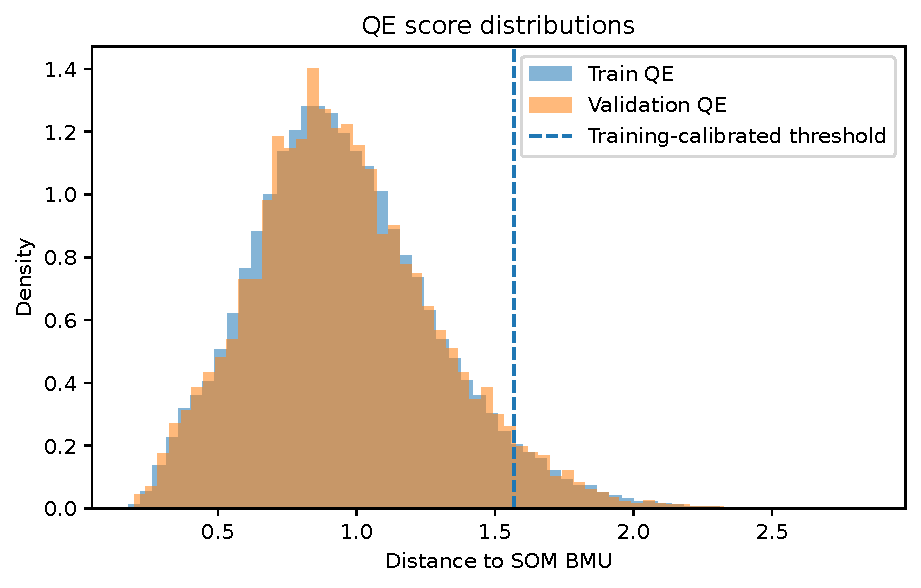
\includegraphics[width=0.82\linewidth]{fig/qe_novelty_detection/qe_score_distribution.pdf}
\caption{Existing MNIST train and validation QE score distributions, with the training-calibrated threshold. This is an in-distribution consistency view, not an OOD discrimination curve.}\label{fig:qe_dist}\end{figure}

\subsection{U-Matrix novelty score}
For SOM neuron $j$ and its grid neighbors $\mathcal N(j)$, the U-Matrix summarizes prototype separations as $U_j=|\mathcal N(j)|^{-1}\sum_{k\in\mathcal N(j)}\|w_j-w_k\|_2$. Each example receives a score derived from its BMU's U-Matrix neighborhood. A high score indicates larger separation among nearby prototypes, not necessarily a large sample-to-prototype distance. The supplied heatmap displays the top 10\% of high U-Matrix regions and uses the 15$\times$15 grid.
\begin{figure}[htbp]\centering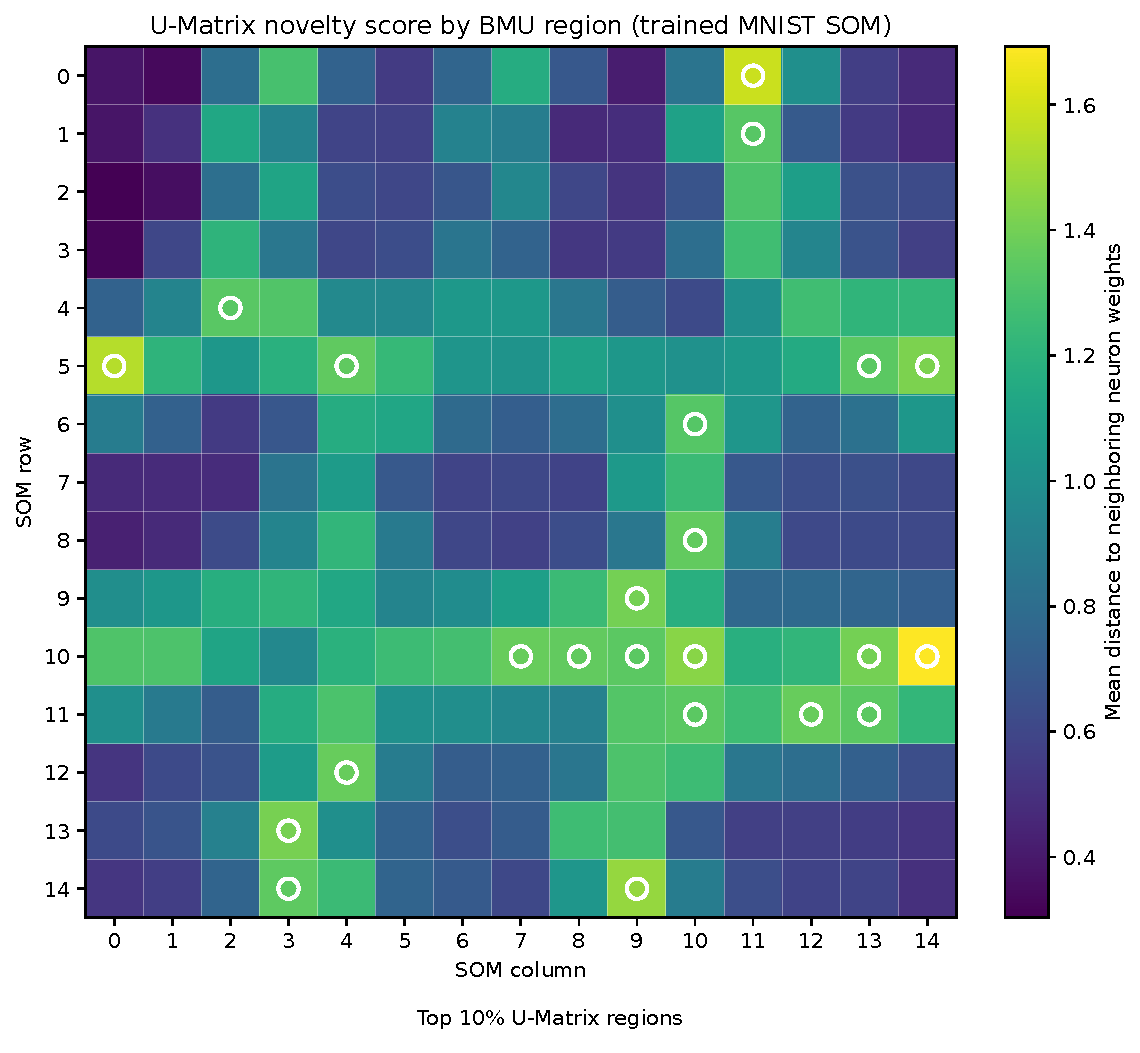
\includegraphics[width=0.92\linewidth]{fig/u_matrix_analysis/u_matrix_novelty_som_grid.pdf}
\caption{U-Matrix novelty values across the trained 15$\times$15 MNIST SOM. Highlighted neurons mark the displayed top 10\% of high-neighborhood-distance regions; these are not labels or evidence of OOD by themselves.}\label{fig:umap}\end{figure}

\subsection{Reference baselines}
The comparison includes Isolation Forest (200 trees, \texttt{max\_samples}=256, contamination 0.05), RBF One-Class SVM ($\nu=0.05$, \texttt{gamma=scale}, 10,000 training embeddings), and an 84--32--16 feature autoencoder trained for 20 epochs (batch size 256, learning rate 0.001). These are recorded settings, not a claim of equal fitting budgets. The autoencoder's reported training loss decreased from 7.21625 to 0.11245, with MNIST validation reconstruction error 0.11097. This training result alone does not establish OOD detection quality.

\section{Measured Results}
\subsection{Comparison on MNIST validation and SVHN test}
AUROC measures ranking discrimination across thresholds; AUPR here treats SVHN/OOD as the positive class. FPR@95TPR is the ROC operating point at 95\% true-positive rate and must \emph{not} be confused with the deployment performance of the frozen QE threshold. The confidence intervals below are those reported in the source artifact using 2,000 bootstrap repetitions. Corresponding AUROC and AUPR point estimates were independently recomputed from the uploaded per-sample score arrays and matched the JSON record.

\begin{table}[htbp]\centering\small
\caption{Recorded five-method OOD results (seed 42; 10,500 MNIST validation negatives and 26,032 SVHN test positives). 95\% bootstrap CI is shown for AUROC; percentages are not used.}
\begin{tabular}{@{}lccc@{}}\toprule
Method & AUROC [95\% CI] & AUPR & FPR@95TPR \\\midrule
QE & 0.9811 [0.9790, 0.9831] & 0.9766 & 0.0453\\
U-Matrix & 0.9696 [0.9670, 0.9721] & 0.9865 & 0.0701\\
Isolation Forest & 0.2383 [0.2307, 0.2456] & 0.5552 & 0.8718\\
One-Class SVM & 0.9604 [0.9581, 0.9627] & 0.9764 & 0.1794\\
Autoencoder & 0.0077 [0.0069, 0.0085] & 0.4979 & 0.9999\\
\bottomrule\end{tabular}\label{tab:measured}\end{table}

The score arrays have exactly the expected number of examples. QE has the highest \emph{reported AUROC} and the smallest \emph{reported FPR@95TPR} of these five methods, while the U-Matrix has the highest \emph{reported AUPR}. These comparisons are descriptive for a single seed and OOD dataset; they do not establish general superiority.

\subsection{QE threshold failure examples}
The recorded QE threshold flagged 25,036 of 26,032 SVHN examples and missed 996, for a source-reported SVHN detection rate of 0.9617 at that frozen threshold. This rate is not FPR@95TPR. Figure~\ref{fig:missed} shows the 20 lowest-QE SVHN examples below the threshold, retained as descriptive examples, not a causal diagnosis of failure.
\begin{figure}[htbp]\centering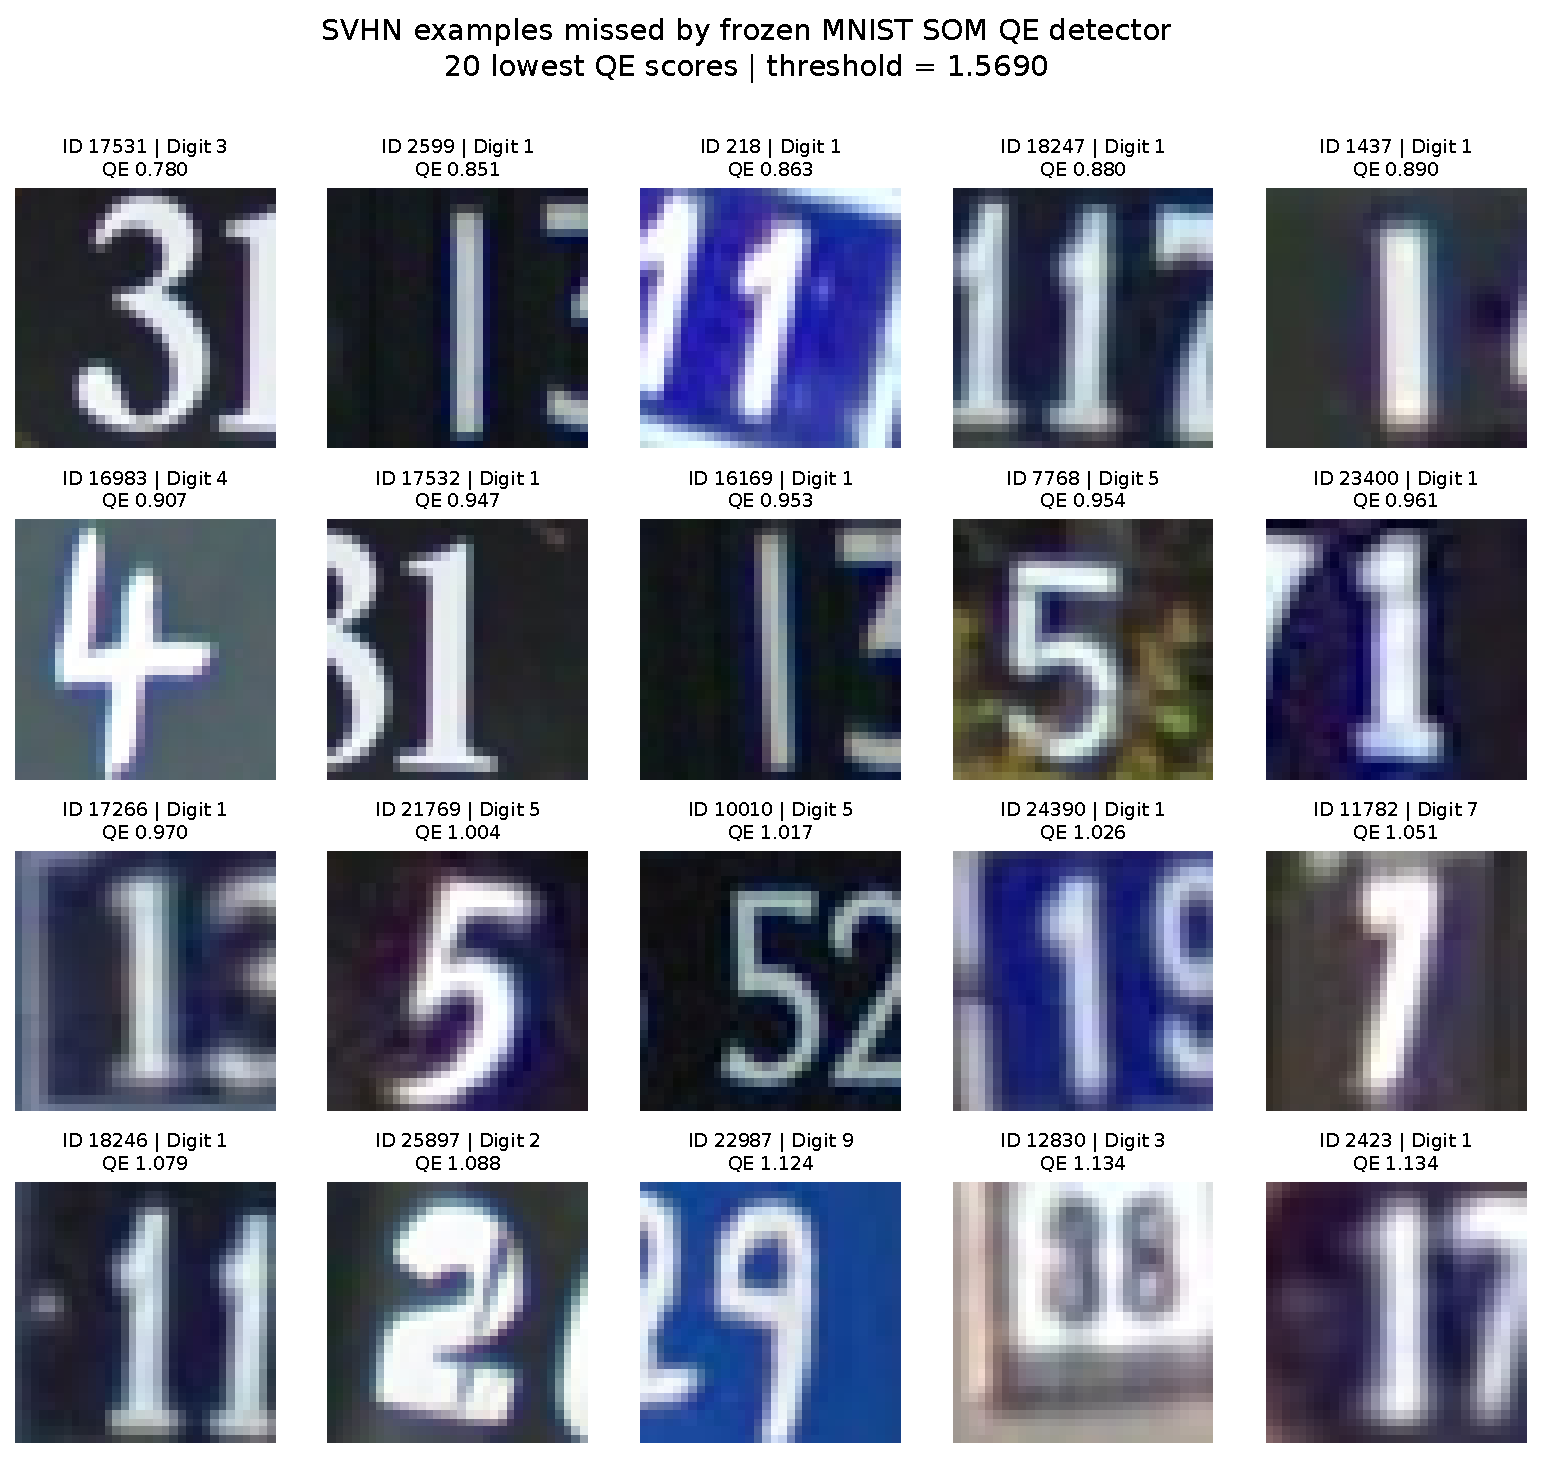
\includegraphics[width=0.98\linewidth]{fig/novelty_benchmark/qe_missed_svhn_examples.pdf}
\caption{Twenty SVHN images with the lowest QE scores under the frozen MNIST SOM detector, all below the recorded threshold of 1.5690. The example identifiers and numeric scores are taken from the supplied figure.}\label{fig:missed}\end{figure}

\subsection{QE and U-Matrix relationship}
The existing MNIST validation scatter shows a Spearman rank correlation of 0.4396 over 10,500 samples (Figure~\ref{fig:scatter}). The moderate positive association is consistent with the scores measuring related yet distinct SOM properties. The scatter alone cannot show which detector is preferable for unseen OOD distributions.
\begin{figure}[htbp]\centering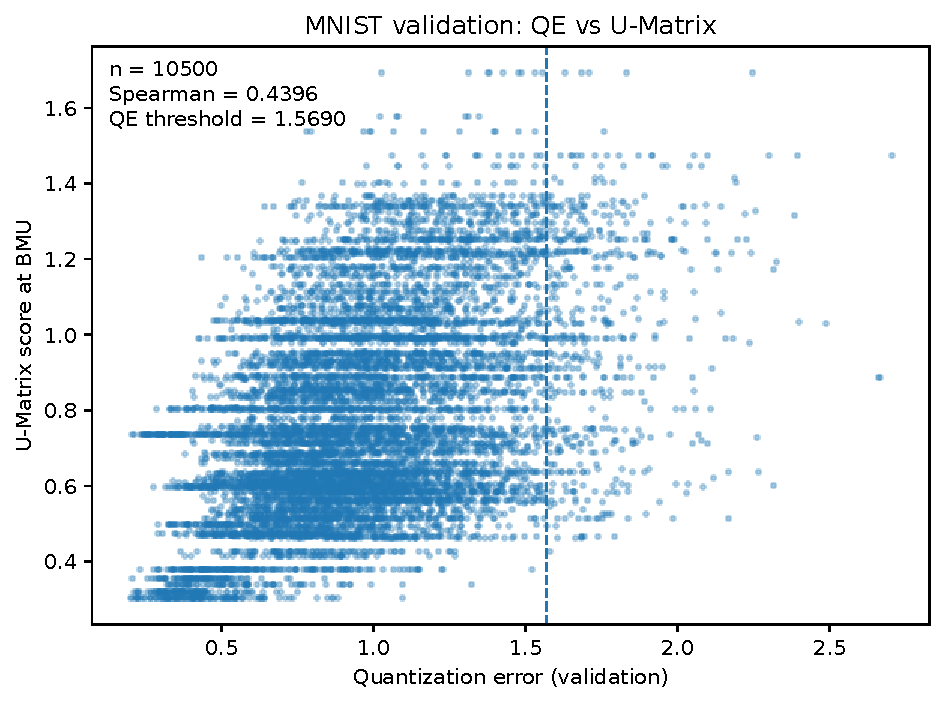
\includegraphics[width=0.90\linewidth]{fig/u_matrix_analysis/qe_u_matrix_validation_initial.pdf}
\caption{MNIST validation QE versus U-Matrix BMU score ($n=10{,}500$; Spearman $\rho=0.4396$), with the recorded QE threshold.}\label{fig:scatter}\end{figure}

\section{Leakage Control and Study Design}
The supplied benchmark JSON states that the CNN and SOM were frozen, training-only MNIST data fitted the classical and autoencoder baselines, and MNIST validation and SVHN test supplied scoring populations. It explicitly states that OOD scores were not used for tuning. This is the \emph{recorded protocol}; this reporting exercise has not independently audited all training logs or code paths. Because the SVHN \emph{test} split has already been scored, it must be treated as observed evaluation evidence, not repurposed as development data. No post-hoc change to threshold, direction, hyperparameters, or selected headline model is justified by these results.

The five methods used unequal fitting sample budgets: One-Class SVM trained on 10,000 versus 49,000 for other learned comparators. Only seed 42 and a single SVHN OOD dataset are recorded. Pre-registered multi-seed validation, fair equal-budget comparisons, null controls, and final locked-test selection documentation remain [TBD]. Planned max-softmax, energy and Mahalanobis baselines also remain [TBD]. If those experiments are added, they require new run IDs, frozen selection criteria, and permitted validation-only development without retroactive claims about an independent test set.

\section{Reproducibility and Quality Controls}
The run ID is \texttt{mnist\_svhn\_five\_method\_comparison\_s42\_initial}; frozen SOM reference and multiple SHA-256 digests are recorded in \texttt{comparison\_metrics.json}. The companion reproducibility record states that a Phase 3 EC2 check yielded 27 passing tests and Ruff passed, while the full repository run yielded 118 passed, three skipped, and three errors related to Phase 1 dataset permissions. An autoencoder rerun matched its reported numeric values in that same EC2 environment, but a full version manifest and saved autoencoder checkpoint were absent. These statements reflect the \emph{uploaded verification record}, not a new CI run.

On the author's Mac, Phase 3 Ruff passed while Phase 3 pytest initially stopped at collection because \texttt{torch} was missing in a Python 3.13 Intel-macOS environment. A separate Python 3.11 virtual environment has been created outside the repository, but a successful fresh Mac pytest result has \emph{not} been supplied. That distinction must be retained until the new test run is observed. No source files or generated research outputs were modified in preparing this report.

\section{Limitations and Interpretation}
Two baseline ranking results require investigation: Isolation Forest AUROC is 0.2383, and autoencoder AUROC is 0.0077 under the reported higher-is-more-novel convention. Independently reversing the existing autoencoder score \emph{for diagnostic analysis only} gives AUROC approximately 0.9923; this is evidence of possible score orientation or distribution-specific reconstruction behavior, \emph{not} an authorized replacement headline score. The corresponding Isolation Forest reversed-direction AUROC is approximately 0.7617. Correcting or redesigning baselines would require a new protocol-compliant run, not rewriting this existing run's outcome.

The unusually high OOD prevalence (26,032 positives out of 36,532 evaluations) influences AUPR; its comparison with a 50\% prevalence or other datasets requires care. The present evidence does not cover multiple OOD benchmarks, calibration of deployable thresholds for every method, or at least five seeds. The U-Matrix heatmap is a topology diagnostic, not a direct heatmap of individual SVHN novelty scores. The strongest supported conclusion is conditional discrimination on this recorded MNIST-validation-versus-SVHN-test experiment, subject to the stated constraints.

\section{Conclusion and Next Steps}
For this recorded single-seed evaluation, QE achieved AUROC 0.9811 and FPR@95TPR 0.0453; U-Matrix achieved AUROC 0.9696 and AUPR 0.9865. The methods reflect different SOM geometry signals and are not interchangeable. Before claiming final Phase 3 completion or transferring these findings to other datasets, the project must record missing control baselines and comparable fitting budgets, verify local tests, establish the final frozen selection protocol and multi-seed uncertainty, and preserve auditable run provenance. This report retains the supplied numbers and original PDF plots without changing the shared project files.

\printbibliography[title={References}]
\end{document}
